\documentclass[11pt,a4paper]{article}

\usepackage[utf8]{inputenc}
\usepackage[T1]{fontenc}
\usepackage{amsmath,amssymb}
\usepackage{graphicx}
\usepackage{booktabs}
\usepackage{enumitem}
\usepackage{geometry}
\usepackage{setspace}
\usepackage{placeins}
\usepackage{microtype}
\usepackage{times}
\usepackage{natbib}
\usepackage[hyphens]{url}
\usepackage{hyperref}

\geometry{margin=0.95in}
\onehalfspacing
\setlength{\emergencystretch}{2em}
\clubpenalty=10000
\widowpenalty=10000
\graphicspath{{figures/}}

\newcommand{\excess}{\mathrm{excess3}}
\newcommand{\Respair}{\mathrm{Res}_{\mathrm{pair}}}
\newcommand{\msalt}[1]{\par\nopagebreak\vspace{1pt}{\footnotesize\textit{Alt text.} #1}\par}

\hypersetup{
  pdftitle={A low-diversity ordinal regime produces the excess3 peak near the logistic accumulation point},
  pdfauthor={Johel Padilla-Villanueva},
  pdfsubject={Preprint, DOI 10.5281/zenodo.22945800},
  pdfkeywords={excess3, ordinal patterns, Feigenbaum accumulation, pairwise residual, coupled logistic maps},
  breaklinks=true,
  colorlinks=false,
  pdfborder={0 0 0}
}

\title{A low-diversity ordinal regime produces the excess3 peak\\
near the logistic accumulation point}

\author{%
Johel Padilla-Villanueva\\
Department of Environmental Health\\
University of Puerto Rico Medical Sciences Campus\\
ORCID: 0000-0002-5797-6931\\
\texttt{johelpadilla@gmail.com}%
}

\date{24 September 2026}

\begin{document}
\maketitle
\begin{center}
DOI: \href{https://doi.org/10.5281/zenodo.22945800}{10.5281/zenodo.22945800}
\end{center}

\begin{abstract}
On four diffusively coupled logistic maps, the hybrid proxy
$\excess=0.6\,\mathrm{Syn}+0.4\,\mathrm{Surp}$ reaches its maximum near
the period-doubling accumulation and is lower in developed chaos. The
geometric reading of that maximum was left as a hypothesis. The same
generator, seeds, and hybrid are decomposed here on a grid of 49 parameter
values, with six realizations at each value. The six-seed mean is largest
at $r=3.5675$, where $\excess=2.378\pm 0.002$ in windows of 13 symbols.
Surprise against independence carries that elevation. The synergy term is
$0.0065\pm 0.0004$ there and attains its own maximum only at $r=3.95$.
Inside the short window the joint occupies $4.11\pm 0.02$ ordinal tuples.
Independent draws from the pairwise maximum-entropy projection of the
invariant joint reproduce the score of independent draws from the joint
itself. The sliding window lies about $0.30$ bits higher because
consecutive symbols are more concentrated than independent samples. The
Kullback--Leibler residual beyond pairwise margins is $0.0003\pm 0.0001$
on the full symbol block at the maximum and $0.192\pm 0.002$ at $r=3.85$,
where the proxy has already fallen. A period-3 window does not repeat the
peak. Lengthening the window from 6 to 312 symbols leaves the accumulation
score near $2.3$ and lowers the chaotic score from about $2.08$ to $0.51$.
The high values form a band, $r\in[3.544,3.595]$, rather than a cusp at the
accumulation point. On this generator the proxy and the irreducible
residual mark different parts of the cascade.
\end{abstract}

\noindent\textbf{Keywords:}
excess3; Bandt--Pompe patterns; Feigenbaum accumulation; pairwise residual;
coupled logistic maps

\vspace{0.6em}
\noindent\textbf{Resumen.}
En cuatro mapas logísticos acoplados, el proxy
$\excess=0.6\,\mathrm{Syn}+0.4\,\mathrm{Surp}$ alcanza su máximo cerca de
la acumulación de doblamiento de periodo. En una rejilla de 49 valores de
$r$, con seis realizaciones, ese máximo está en $r=3.5675$ y vale
$2.378\pm 0.002$ para ventanas de 13 símbolos. La elevación la lleva la
sorpresa frente a la independencia. La sinergia vale ahí
$0.0065\pm 0.0004$ y solo crece más adelante. La ventana ocupa
$4.11\pm 0.02$ tuplas ordinales conjuntas. La proyección de máxima
entropía por pares reproduce el valor de extracciones independientes de la
ley conjunta; la ventana deslizante queda unos $0.30$ bits por encima
porque los símbolos consecutivos están más concentrados. El residuo de
Kullback--Leibler más allá de los pares es $0.0003\pm 0.0001$ en el bloque
completo del máximo y $0.192\pm 0.002$ en $r=3.85$, donde el proxy ya
bajó. La ventana de periodo~3 no repite el pico. Alargar la ventana
mantiene el pico y agranda el contraste con el caos. En este generador el
proxy y el residuo irreducible marcan tramos distintos de la cascada.

\section{Introduction}
\label{sec:intro}

A critical transition is often described through the growth of variance
and lag-1 autocorrelation \citep{Scheffer2009}. An ordinal reading asks a
different question: whether the joint order of several series is being
reorganized \citep{BandtPompe2002,Padilla2026framework}. In that reading,
Systemic Tau summarizes pairwise rank concordance, and a discrete clock is
built from nested ordinal conjunctions. The third level of the clock is
the residual of the joint ordinal law beyond pairwise margins. The hybrid
$\excess$ was specified so that a short window could be scored when that
residual is costly to compute \citep{Padilla2026excess3,Padilla2026nested}.
The weights $0.6$ and $0.4$ are a declared design choice. They were not
fitted to the logistic suite.

On the published cascade of diffusively coupled logistic maps,
$\excess$ is higher at $r=3.85$ than at $r=3.30$, and its grid maximum
lies near the accumulation point rather than in developed chaos, at about
$2.38$ \citep{Padilla2026framework}. The manuscript records that location
as an observation. The geometric account attached to it --- a high-period
orbit concentrated on a few joint symbols, still describable by pairs ---
is stated there as a hypothesis.

This paper tests that hypothesis. The test uses the published generator,
the published seeds, and the published hybrid, on a grid refined through
the accumulation band. Three comparisons are fixed in advance. The first
splits the hybrid into $\mathrm{Syn}$ and $\mathrm{Surp}$. The second
asks whether the pairwise maximum-entropy law already produces the score.
The third asks whether the peak survives when the window is lengthened,
and whether a period-3 window repeats it. The residual
$\Respair$ is reported beside the proxy and is not replaced by it.

\section{Estimators}
\label{sec:estimators}

Let $S_t\in\{0,\ldots,5\}^4$ be the joint Bandt--Pompe symbol of order
$m=3$ and delay $1$ at time $t$ \citep{BandtPompe2002}. In a window of
length $w$, write $p$ for the empirical law of the joint symbol and
$p_i$ for its marginals. Total correlation, in bits, is
\begin{equation}
\mathrm{TC}
=\sum_{i=1}^{4} H(p_i)-H(p).
\end{equation}
The pairwise summary used by the proxy is $(4-1)$ times the mean pairwise
mutual information. Synergy in this construction is the nonnegative excess
of total correlation over that summary,
\begin{equation}
\label{eq:syn}
\mathrm{Syn}
=\bigl[\mathrm{TC}-(d-1)\,\overline{I}_{\mathrm{pair}}\bigr]_+,
\qquad d=4.
\end{equation}
Surprise retains the positive part of the log-ratio against independence,
\begin{equation}
\label{eq:surp}
\mathrm{Surp}
=\sum_{s} p(s)\,
\bigl[\log_2 p(s)-\log_2 p_{\mathrm{ind}}(s)\bigr]_+,
\end{equation}
with $p_{\mathrm{ind}}(s)=\prod_i p_i(s_i)$ and the marginal probability
floored at $10^{-9}$ in the published implementation. The hybrid is
\begin{equation}
\label{eq:excess}
\excess=0.6\,\mathrm{Syn}+0.4\,\mathrm{Surp}.
\end{equation}
These names are local to the proxy. They are not the synergy and
redundancy atoms of a partial information decomposition
\citep{Williams2010}.

The strong residual is a different functional. Let $P^{(2)}$ be the
maximum-entropy law with the same pairwise margins as $p$, obtained by
iterative proportional fitting. Then
\begin{equation}
\label{eq:res}
\Respair
=D_{\mathrm{KL}}\bigl(p\,\Vert\,P^{(2)}\bigr),
\end{equation}
in bits. A positive value of $\excess$ does not imply a positive value of
$\Respair$. Surprise is large for a joint that is far from independence,
including a joint that pairs already explain.

\section{Protocol}
\label{sec:protocol}

The system is the diffusively coupled logistic family used for the
published cascade \citep{Kaneko1992,Padilla2026framework}. Four
coordinates obey
\begin{equation}
\label{eq:map}
\begin{aligned}
f_i(t)&=r\,x_i(t)\bigl(1-x_i(t)\bigr),\\
x_i(t+1)
&=(1-\varepsilon)\,f_i(t)
+\varepsilon\,\overline{f}_{-i}(t)
+\xi_i(t),
\end{aligned}
\end{equation}
with the mean $\overline{f}_{-i}$ taken over the other three logistic
images, $\varepsilon=0.05$, and $\xi_i(t)$ independent Gaussian noise of
standard deviation $0.003$. Each coordinate is then clipped to $[0,1]$.
The initial condition is uniform on $[0.2,0.8]$. Four hundred steps are
discarded and $2200$ steps are retained. The seed of realization $k$ at
parameter $r$ is
\begin{equation}
\label{eq:seed}
10000+\lfloor 10000\,r\rfloor+17k,
\qquad k=0,\ldots,5.
\end{equation}
After the embedding, each series contains $2198$ joint symbols.

The parameter grid is the 32-point cascade grid, union a uniform grid of
19 values on $[3.545,3.590]$, restricted to $[3.05,3.98]$. Forty-nine
distinct values remain. The conventional accumulation value of the
logistic family is $r_\infty=3.5699456$
\citep{Feigenbaum1978,Feigenbaum1983}. The nearest grid point is
$r=3.569946$. The period-3 window is represented by $r=3.828427$.

For windows of length $13$ the hybrid is the mean over every consecutive
window, which is the published abundance. For every other length in
$\{6,8,10,13,20,26,40,52,78,104,156,208,312\}$
the same mean is taken on about $160$ evenly spaced windows, the stride
being the smallest integer that yields at most that count. The full-block
scores use all $2198$ symbols as one window. Means and standard errors
below are taken across the six seeds. The standard error uses the sample
standard deviation with divisor $5$.

Two Monte Carlo controls use the invariant joint of each series. Eighty
sequences of length $13$ are drawn independently from $p$, and eighty from
$P^{(2)}$, with the random generator seeded by the series seed plus $901$.
A local control repeats the comparison inside $36$ evenly spaced windows
of length $13$, with four draws from that window's own $p$ and four from
its pairwise projection. The film strip in Figure~\ref{fig:film} is one
realization per station: the seed whose mean number of distinct 13-symbol
tuples is closest to the six-seed mean, and, inside that series, a run of
16 symbols whose support is closest to the series mean.

The window-13 means at $r=3.30$ and $r=3.85$ agree with the cascade
archive to the stored digits, $1.757509$ and $1.863299$. At every station
the stored means satisfy
$0.6\,\mathrm{Syn}+0.4\,\mathrm{Surp}=\excess$
to the precision of the archive.

\section{Results}
\label{sec:results}

\subsection{The maximum is a band, and Surp carries it}
\label{sec:band}

Figure~\ref{fig:decomp} shows the three scores along the grid.
Table~\ref{tab:stations} lists the stations used below. The largest
six-seed mean of $\excess$ is $2.378\pm 0.002$ at $r=3.5675$. The
neighboring station $r=3.566168$, the location cited for the cascade
maximum, has mean $2.378\pm 0.003$. At the nearest grid point to
$r_\infty$ the mean is $2.343\pm 0.032$. Across the 33 stations in
$[3.544,3.595]$, 29 means exceed $2.30$. The lowest mean in that band is
$2.204$ and the highest is $2.378$.

Leave-one-seed maxima of the mean fall at $r=3.566168$ once, at
$r=3.5675$ four times, and at $r=3.575$ once. All six lie inside the same
band. The maximum is the top of a plateau.

At $r=3.5675$ the two pieces of the hybrid are
$\mathrm{Syn}=0.0065\pm 0.0004$ and
$\mathrm{Surp}=5.936\pm 0.004$. Their weighted contributions are
$0.0039$ and $2.374$ bits. The elevation above developed chaos at
$r=3.85$, where $\excess=1.863\pm 0.004$, is $0.515$ bits. The Surp term
contributes $+0.566$ bits to that difference and the Syn term contributes
$-0.051$ bits. Along the 49 grid means, the correlation of $\excess$ with
$\mathrm{Surp}$ is $0.999$, with $\mathrm{Syn}$ it is $-0.778$, and with
the number of distinct tuples it is $-0.975$. The largest Syn on the grid
is $0.118$ at $r=3.95$.
\FloatBarrier

\begin{figure}[tp]
\centering
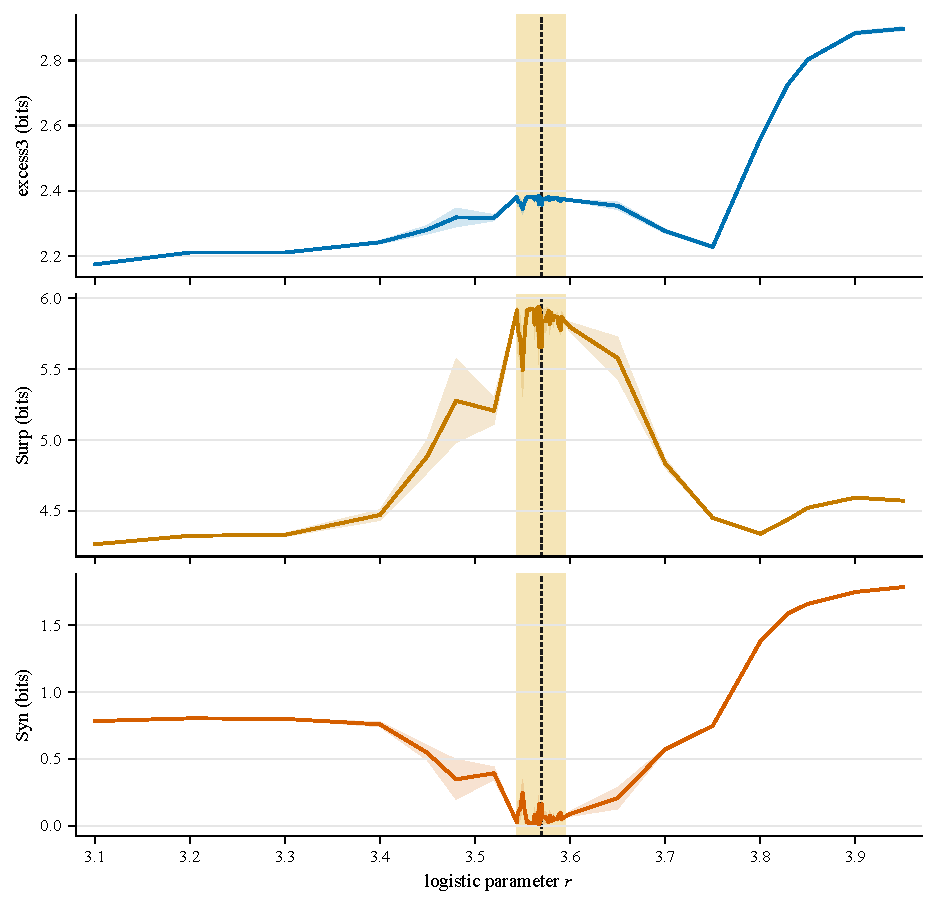
\includegraphics[width=\textwidth]{fig2_decomposition.pdf}
\caption{Window-13 scores along the logistic parameter. Curves are
six-seed means and shading is the standard error. The band marks
$r\in[3.544,3.595]$. The dashed line is $r_\infty=3.5699456$.
$\mathrm{Surp}$ follows $\excess$. $\mathrm{Syn}$ is near zero inside
the band and is largest at the right edge of the grid.}
\label{fig:decomp}
\msalt{Three stacked curves against the logistic parameter. Excess3 and surprise both rise to a plateau near 3.57 and then fall. Synergy is near zero on that plateau and rises only after 3.75.}
\end{figure}

\begin{table}[t]
\centering
\footnotesize
\setlength{\tabcolsep}{3.2pt}
\caption{Six-seed means at nine stations. The standard error of the mean
is in parentheses. Tuples, visits, and modal mass refer to windows of length 13.
$\Respair$ is the Kullback--Leibler residual of the full symbol block.}
\label{tab:stations}
\resizebox{\textwidth}{!}{%
\begin{tabular}{@{}llrrrrrrr@{}}
\toprule
$r$ & regime & $\excess$ & Syn & Surp & tuples & visits & modal & $\Respair$ \\
\midrule
3.30000 & period 2 & 2.210 (0.002) & 0.7974 (0.0051) & 4.329 (0.012) & 11.39 (0.05) & 1.15 & 0.147 & 0.0024 (0.0004) \\
3.44949 & period 4 & 2.280 (0.013) & 0.5454 (0.0546) & 4.882 (0.115) & 8.91 (0.55) & 1.64 & 0.190 & 0.0018 (0.0006) \\
3.54409 & period 8 & 2.381 (0.002) & 0.0242 (0.0109) & 5.915 (0.021) & 4.20 (0.09) & 3.16 & 0.302 & 0.0005 (0.0002) \\
3.56617 & near $r_\infty$ & 2.383 (0.000) & 0.0145 (0.0043) & 5.935 (0.007) & 4.12 (0.03) & 3.20 & 0.304 & 0.0005 (0.0003) \\
3.95000 & grid maximum & 2.897 (0.006) & 1.7817 (0.0096) & 4.571 (0.008) & 12.79 (0.02) & 1.02 & 0.090 & 0.1816 (0.0025) \\
3.56995 & $r_\infty$ & 2.375 (0.007) & 0.0619 (0.0442) & 5.845 (0.083) & 4.51 (0.36) & 3.04 & 0.293 & 0.0031 (0.0028) \\
3.82843 & period-3 window & 2.723 (0.007) & 1.5823 (0.0094) & 4.435 (0.008) & 12.56 (0.02) & 1.04 & 0.101 & 0.1938 (0.0052) \\
3.85000 & developed chaos & 2.802 (0.005) & 1.6570 (0.0053) & 4.521 (0.010) & 12.62 (0.02) & 1.04 & 0.098 & 0.1921 (0.0016)
\\
\bottomrule
\end{tabular}}
\msalt{A table of nine logistic parameter values. Excess3 and surprise are highest near r = 3.5675, where about four joint tuples appear. The full-block residual is near zero there and near 0.19 in the period-3 window and in developed chaos.}
\end{table}

\subsection{The joint support collapses}
\label{sec:support}

Figure~\ref{fig:support} places the support next to the block residual.
At the grid maximum a window of 13 symbols contains
$4.11\pm 0.02$ distinct joint tuples, visited $3.20$ times on average,
with modal mass $0.304$. At $r=3.30$ the same window contains
$11.39\pm 0.05$ tuples. At $r=3.85$ it contains $12.62\pm 0.02$, visited
$1.04$ times, with modal mass $0.098$.

Figure~\ref{fig:film} shows sixteen consecutive symbols from the
representative realization at each of those three stations. At
$r=3.5675$ the segment is the cycle of four joint symbols
$1,2,3,4$, repeated four times. The integers are the order of first
appearance in the segment. They label distinct 4-tuples of permutation
indices; they are not comparable across panels, and they are not
themselves the Bandt--Pompe ranks. At $r=3.30$ the segment uses eleven
joint symbols. At $r=3.85$ it uses thirteen.
\FloatBarrier

\begin{figure}[tp]
\centering
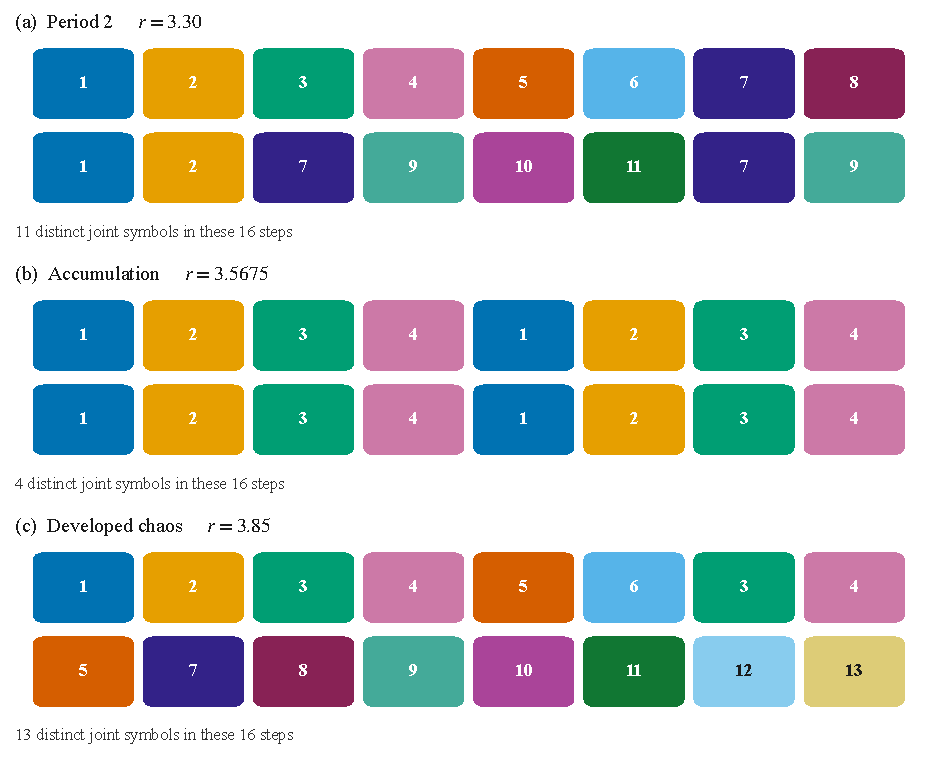
\includegraphics[width=\textwidth]{fig1_filmstrip.pdf}
\caption{Sixteen consecutive joint symbols, read left to right and then
onto the second row. The displayed integer is the order of first
appearance within the segment. The segment is chosen by the rule in
Section~\ref{sec:protocol}.
(a)~Period~2 uses eleven joint symbols.
(b)~At the grid maximum the same four joint symbols repeat.
(c)~Developed chaos uses thirteen joint symbols in the same length.}
\label{fig:film}
\msalt{Three pairs of colored rows. The middle pair repeats the colors and numbers 1, 2, 3, 4. The top and bottom pairs introduce many more colors.}
\end{figure}

\begin{figure}[tp]
\centering
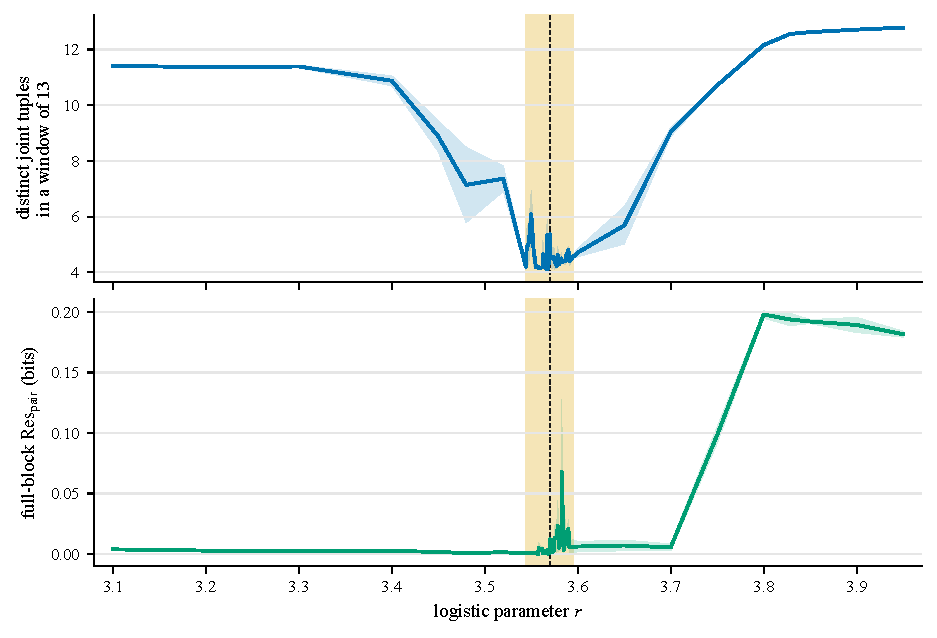
\includegraphics[width=\textwidth]{fig3_support_residual.pdf}
\caption{Support and block residual along $r$. Shading, band, and dashed
line are as in Figure~\ref{fig:decomp}. The number of distinct joint
tuples in a window of 13 is smallest inside the band. The full-block
residual stays near zero there, apart from isolated grid points whose
standard error is comparable to the mean: at $r=3.582612$ the residual
mean is $0.068$ with standard error $0.059$. The residual then rises and
reaches $0.198\pm 0.003$ at $r=3.80$.}
\label{fig:support}
\msalt{Two stacked curves. The count of distinct joint tuples falls to about four inside the yellow band and then rises past twelve. The full-block residual stays near zero through that band and rises to about 0.20 after r = 3.75.}
\end{figure}

The block residual does not follow the proxy. At $r=3.5675$ it is
$0.0003\pm 0.0001$. At $r=3.85$ it is $0.192\pm 0.002$, and its grid
maximum is $0.198\pm 0.003$ at $r=3.80$. The full-block hybrid itself
remains high through the accumulation band. Its grid maximum is $2.298$
at $r=3.5575$. At $r=3.85$ the full-block hybrid has fallen to
$0.174\pm 0.003$.
\FloatBarrier

\subsection{Pairs reproduce the stationary score}
\label{sec:pairs}

Table~\ref{tab:controls} compares the sliding window with the two
independent-draw experiments. At the grid maximum, draws from the
empirical joint $p$ score $2.073\pm 0.067$, and draws from $P^{(2)}$
score $2.088\pm 0.062$. The ratio of the pairwise score to the sliding
score is $0.878$. At $r=3.85$ the same ratio is $0.910$. The pairwise
projection therefore accounts for the excess3 of the invariant joint.
What it does not account for is the extra concentration of consecutive
symbols: the sliding mean exceeds the independent draws from $p$ by
$0.305\pm 0.067$ bits at the maximum, about one eighth of the sliding
score. Those sliding windows occupy $4.11$ tuples, while the independent
draws from the same $p$ occupy $5.54$.

Inside single windows the comparison is tighter. At the grid maximum the
gap between a window and draws from its own pairwise projection is
$0.164\pm 0.002$, and the gap against draws from that window's own $p$ is
$0.146\pm 0.006$. The two gaps agree at the scale of the Monte Carlo
error. At $r=3.85$ the local pairwise gap is $-0.035\pm 0.008$. The short
window does not contain a residual beyond pairs above the sampling
fluctuation of a 13-symbol table.

\begin{table}[t]
\centering
\small
\setlength{\tabcolsep}{6pt}
\caption{Grid maximum against developed chaos. Entries are six-seed means
$\pm$ the standard error. Independent draws are eighty sequences of length
13. Local gaps use 36 windows and four draws each.}
\label{tab:controls}
\begin{tabular}{@{}lcc@{}}
\toprule
quantity & $r=3.5675$ & $r=3.85$ \\
\midrule
excess3, $w=13$ & 2.383 $\pm$ 0.0004 & 2.802 $\pm$ 0.005 \\
Syn & 0.0137 $\pm$ 0.0021 & 1.6570 $\pm$ 0.0053 \\
Surp & 5.936 $\pm$ 0.004 & 4.521 $\pm$ 0.010 \\
distinct tuples, $w=13$ & 4.11 $\pm$ 0.02 & 12.62 $\pm$ 0.02 \\
visits per tuple & 3.20 & 1.04 \\
modal mass & 0.304 & 0.098 \\
iid draws from $P$ & 2.161 $\pm$ 0.033 & 2.629 $\pm$ 0.020 \\
iid draws from $P^{(2)}$ & 2.174 $\pm$ 0.025 & 2.639 $\pm$ 0.012 \\
sliding minus iid $P$ & 0.221 $\pm$ 0.033 & 0.173 $\pm$ 0.021 \\
local gap vs.\ $P^{(2)}$ & 0.225 $\pm$ 0.005 & 0.340 $\pm$ 0.010 \\
local gap vs.\ own $P$ & 0.206 $\pm$ 0.006 & 0.325 $\pm$ 0.013 \\
full-block excess3 & 2.336 $\pm$ 0.054 & 0.316 $\pm$ 0.005 \\
full-block $\mathrm{Res}_{\mathrm{pair}}$ & 0.0003 $\pm$ 0.0001 & 0.1921 $\pm$ 0.0016 \\
excess3, $w=312$ & 2.375 $\pm$ 0.008 & 1.135 $\pm$ 0.011 \\
distinct tuples, $w=312$ & 6.55 $\pm$ 0.2 & 199.5 $\pm$ 1.2
\\
\bottomrule
\end{tabular}
\msalt{A two-column comparison of the accumulation maximum and developed chaos. Surprise, repeated tuples, and the sliding-window score are higher at the maximum. Synergy and the full-block residual are higher in chaos. Independent draws from the joint and from its pairwise projection agree with each other in both columns.}
\end{table}

\subsection{The peak survives a longer window}
\label{sec:window}

Figure~\ref{fig:windows} extends the hybrid from length 6 to length 312.
At $r=3.5675$ the mean is $2.326$ at length 6, $2.378$ at length 13, and
$2.312\pm 0.027$ at length 312. At that last length the accumulation
series still occupies only $6.5\pm 0.2$ joint symbols, with $55.8$ visits
per occupied tuple. At $r=3.85$ the mean falls from $2.078$ at length 6
through $1.863$ at length 13 and $0.912$ at length 104 to
$0.514\pm 0.006$ at length 312, where the window occupies
$199.5\pm 1.2$ symbols and only $1.57$ visits per tuple. Lengthening the
window enlarges the contrast. It does not create the peak.

The period-3 station $r=3.828427$ follows the chaotic curve. Its
window-13 hybrid is $1.832\pm 0.003$, its support is $12.56\pm 0.02$
tuples, its synergy is $0.096\pm 0.001$, and its block residual is
$0.194\pm 0.005$. A periodic window is not, by itself, the accumulation
peak.

Period~2 behaves in a third way. By length 312 its joint support has
saturated at 32 symbols and $\excess$ has leveled at $1.224$, between the
accumulation plateau and the chaotic decline. The period-8 station
$r=3.54409$ is already inside the high band: $\excess=2.368\pm 0.008$
and the short window holds $4.20\pm 0.09$ tuples.
\FloatBarrier

\begin{figure}[tp]
\centering
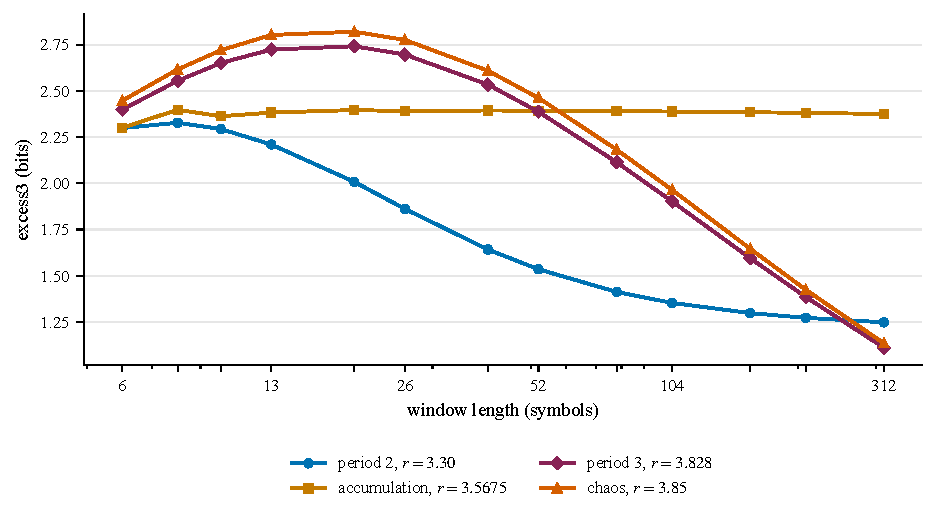
\includegraphics[width=\textwidth]{fig4_windows.pdf}
\caption{The hybrid against window length at four stations. Points are
six-seed means. Lengths above 13 use about 160 evenly spaced windows.
The accumulation curve stays near $2.3$. The period-3 and chaotic curves
fall together toward $0.5$. Period~2 falls and then levels off.}
\label{fig:windows}
\msalt{A log-scaled plot of excess3 against window length. The accumulation curve is nearly flat near 2.3. Period 2 declines and flattens near 1.2. Period 3 and developed chaos decline together to about 0.5 at window length 312.}
\end{figure}

\FloatBarrier
\section{Discussion}
\label{sec:discussion}

The measurement closes the geometric hypothesis on this ensemble. Near
accumulation the orbit of the joint symbol lives on about four tuples.
Those tuples are far from an independent product, so $\mathrm{Surp}$ is
large, and the declared hybrid follows $\mathrm{Surp}$. The same joint is
still close to its pairwise maximum-entropy projection, so $\Respair$ on
the long block is indistinguishable from zero at the reported precision.
Developed chaos widens the support, lowers $\mathrm{Surp}$, and is the
region in which the block residual becomes nonzero. Synergy, as defined
by equation~\eqref{eq:syn}, is the term that rises in that later region,
and on this grid it never sets the location of the hybrid maximum.

The two quantities therefore mark different stations of the same cascade.
A reading that takes the peak of $\excess$ as the place where ordinal
structure beyond pairs is strongest points to the accumulation band. A
reading that takes $\Respair>0$ as that place points to developed chaos,
after the proxy has fallen. The foundations manuscript already separates
the proxy from the residual and already distinguishes a common-driver
geometry, in which surprise is high and the pairwise residual is not, from
a higher-order joint \citep{Padilla2026framework}. The accumulation band
of this coupled logistic system is the first of those geometries. The
chaotic stations are where the second geometry begins to register in the
block residual.

Two smaller facts keep the statement from being sharper than the ensemble.
First, consecutive windows are more concentrated than independent draws
from the invariant joint, by about $0.30$ bits at the maximum. That is a
real temporal contribution. It is smaller than the surprise of the joint,
and the local 13-symbol comparison does not resolve a pairwise gap beyond
the resampling error of the window. Second, one grid point inside the
band, $r=3.582612$, has a block-residual mean of $0.068$ with standard
error $0.059$. Isolated seeds can move a single station. They do not move
the six-seed maximum of the residual, which remains at $r=3.80$.

The scope is the generator in equation~\eqref{eq:map}: four coordinates,
coupling $0.05$, noise level $0.003$, embedding order $3$, and the six
seeds in equation~\eqref{eq:seed}. The weights in equation~\eqref{eq:excess}
are the published weights. Because $\mathrm{Syn}$ is three orders of
magnitude smaller than $\mathrm{Surp}$ at the maximum, a convex
combination that still gives $\mathrm{Surp}$ positive weight keeps the
maximum on the surprise curve; the paper does not refit the weights. The
result does not derive the operational concordance bands used elsewhere in
the framework, and it does not transfer the peak, or the delayed rise of
$\Respair$, to other couplings, other dimensions, or series measured in
the field. Early-warning comparisons with variance and lag-1
autocorrelation remain those of the cascade study.

\section{Conclusion}
\label{sec:conclusion}

On this coupled logistic cascade, $\excess$ peaks near accumulation
because the joint ordinal symbol repeats a handful of tuples and those
tuples are far from independence. The part of the construction that is
meant to see beyond pairs is quiet there. It becomes visible later, in
developed chaos, after the proxy has come down. The period-3 window
follows that later regime. A longer window preserves the peak and widens
its contrast with chaos.

\section*{Author declarations}

\paragraph{Conflict of interest.}
The author has no conflict of interest to disclose.

\paragraph{Ethics approval.}
Ethics approval is not required. The study uses simulated series only.

\paragraph{Author contribution.}
Johel Padilla-Villanueva: conceptualization, methodology, software, formal
analysis, and writing.

\section*{Data availability}
This article is archived at
\url{https://doi.org/10.5281/zenodo.22945800}.
The generator, the seeds, and the estimators are those of the cascade in
\citet{Padilla2026framework} and of nested-recd~0.2.2
\citep{Padilla2026nested}. The decomposition archived for this article is the run of
24~September 2026. The files
\path{peak_flat_20260924_145527.csv},
\path{peak_agg_20260924_145527.csv}, and
\path{peak_results_20260924_145527.json}
accompany this deposit and the repository
\url{https://github.com/johelpadilla/excess3}
under \path{accumulation/data/}.
They were produced by \path{scripts/peak_rinf_decompose.py}.
The figures and the numeric tables were drawn from that archive by
\path{make_figures.py}.
The cascade and diagnostic scripts of the foundations study are
\path{cascade_r_sweep.py} and \path{res_pair_diagnostics.py}.

\bibliographystyle{plainnat}
\bibliography{references}

\end{document}
